\documentclass{beamer}

\usepackage[T1]{fontenc}
\usepackage[utf8]{inputenc}
\usepackage[frenchb]{babel}
\usepackage{eurosym}

\usepackage{graphicx}

% --------- BEGIN STYLE BEAMER ---------
\usetheme{Madrid}
\definecolor{ECNBleu}{HTML}{102648}
\definecolor{ECNJaune}{HTML}{FAB600}

\setbeamercolor{frametitle}{bg=ECNBleu,fg=white} %le titre de la frame, en haut
\setbeamercolor{title in head/foot}{bg=ECNJaune,fg=ECNBleu} %barre bas, milieu
\setbeamercolor{author in head/foot}{bg=ECNBleu,fg=ECNJaune} %barre bas, gauche
\setbeamercolor{date in head/foot}{bg=ECNBleu,fg=ECNJaune} %barre bas, droit
\setbeamercolor{section in head/foot}{bg=ECNJaune,fg=ECNBleu} %haut gauche
\setbeamercolor{subsection in head/foot}{bg=ECNBleu,fg=ECNBleu} %haut droite
\setbeamercolor{title}{bg=ECNBleu,fg=white}
\setbeamercolor{block title}{fg=white,bg=ECNBleu}

%\setbeamercolor{normal text}{bg=IUTBleuFonce} %texte
\setbeamercolor{item}{bg=ECNBleu}
\setbeamercolor{subitem}{bg=ECNJaune}
\setbeamercolor{description item}{fg=couleurEmph}
\setbeamercolor{section in toc}{fg=ECNBleu}
%\setbeamercolor{subsubitem}{bg=IUTBleuFonce}

%structure (eq emph dans beamer)
\setbeamercolor{emph}{fg=couleurEmph}
% ----------------------------

\usepackage{listings}

\lstdefinestyle{customc}{
  belowcaptionskip=1\baselineskip,
  breaklines=true,
  frame=L,
  xleftmargin=\parindent,
  language=C,
  showstringspaces=false,
  basicstyle=\tiny\ttfamily,
  keywordstyle=\bfseries\color{green!40!black},
  commentstyle=\itshape\color{purple!40!black},
  identifierstyle=\color{blue},
  stringstyle=\color{orange},
}

\lstset{escapechar=@,style=customc}

\newenvironment<>{questionblock}[1]{%
\setbeamercolor{block title}{bg=ECNJaune,fg=ECNBleu}%
\begin{block}#2{#1}}{\end{block}}

\title[GPGPU]{Programmation sur Processeur Graphique}
\subtitle[\ldots]{---\\Guide : Utilisation des Jetson nano}
\author[P.-E. Hladik]{Pierre-Emmanuel Hladik\\\tiny pierre-emmanuel.hladik@ec-nantes.fr}
\institute[Centrale Nantes]{}
%{\tiny\date{\today}}
%\logo{
\titlegraphic{
	\flushleft
\includegraphics[width=3cm]{./LogoCN_RVB}
}

\begin{document}

 \frame{\titlepage}
 
 % --------- Princiep ---------
\begin{frame}[plain]
\frametitle{Principe et outils}

\begin{block}{Connexion}
	Vous travailler à distance sur un Jetson Nano. Pour cela, vous connecterez votre PC via une connexion Ethernet à la Jetson, puis vous établirez un pont ssh (un serveur DHCP est installé sur la Jetson).
\end{block}

\begin{block}{IDE}
	Afin de faciliter le travail (et pour uniformiser les installations), vous allez passer par  l'IDE \href{https://code.visualstudio.com}{{\bf Visual Studio Code}} en mode \href{https://code.visualstudio.com/docs/remote/remote-overview}{Remote} (compilation à distance). %Une vidéo est disponible sur \href{https://moodle.insa-toulouse.fr/enrol/index.php?id=1651}{moodle} qui explique comme installer cet éditeur et comment ajouter les extensions nécessaires.
\end{block}
\end{frame}
% ----------------------------

 % --------- Installation VS Code ---------
\begin{frame}[plain]
\frametitle{Installation VS Code}

\begin{block}{}
Téléchargez votre installateur pour VS Code depuis :
\href{https://code.visualstudio.com/download}{https://code.visualstudio.com/download}
\end{block}

{\center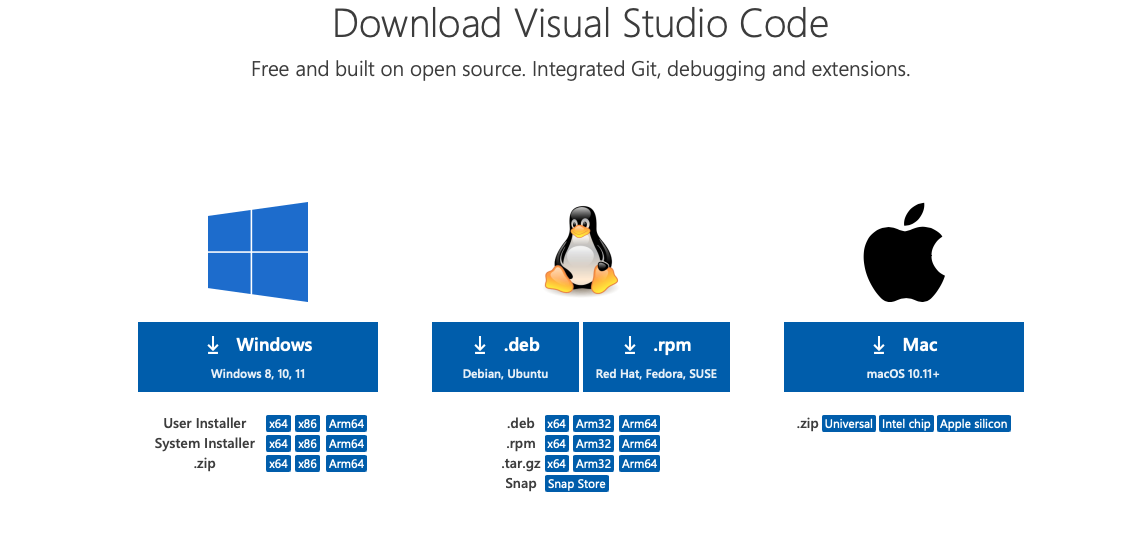
\includegraphics[width=\textwidth]{./figures-pdf/vs_code_install.png}}

\end{frame}
% ----------------------------

 % --------- Installation extension remote ---------
\begin{frame}[plain]
\frametitle{Installation du plugin Remote-SSH}

\begin{itemize}
	\item Lancez VS Code et allez dans l'Extension Market (icône à gauche en bas qui ressemble à quatre carrés dans une boîte avec le carré supérieur droit qui explose).

	\item tapez {\bf Remote-SSH} dans la barre de recherche d’Extensions Marketplace. Lorsque vous trouvez le plugin, sélectionnez-le et cliquez ensuite sur le bouton vert {\bf Install} pour installer l’extension.
\end{itemize}

{\center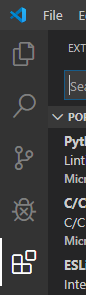
\includegraphics[scale=0.4]{./figures-pdf/BRp46yv}}

\end{frame}
% ----------------------------

 % --------- Installation extension remote ---------
\begin{frame}[plain]
\frametitle{Se connecter à la carte}

\begin{alertblock}{}
Attention il est nécessaire d'avoir un accès à internet pour pouvoir mettre en place le pont entre votre PC et le Jetson. Assurez-vous que vous avez bien une connexion wifi active.
\end{alertblock}

\begin{alertblock}{Pour OS X}
Attention il faut que vous connexion wifi soit prioritaire par rapport à votre connexion Ethernet.  Allez dans Préférences Système->Réseau->Avancé...->Wi-Fi et vérifier l'ordre de priorité.
\end{alertblock}

\begin{itemize}
	\item Depuis VS Code, cliquez sur le bouton vert {\bf Open a remote window} dans le coin inférieur gauche et sélectionnez {\bf Remote-SSH : Connect to Host...}
	\item Saisissez l'adresse IP de la carte : pehladik@192.168.1.100 (l'utilisateur est pehladik)
	\item Saisissez le mot de passe : kywy
\end{itemize}

\end{frame}
% ----------------------------

 % --------- Installation extension remote ---------
\begin{frame}[plain]
\frametitle{Se connecter à la carte}


Pour configurer de manière définitive la connexion, vous pouvez :
\begin{itemize}
	\item Cliquez sur le bouton vert {\bf Open a remote window} dans le coin inférieur gauche et sélectionnez {\bf Remote-SSH : Open Configuration File...}
	\item Saisissez les informations concernant la connexion ssh.
\end{itemize}

\end{frame}
% ----------------------------

\end{document}